%
% introduction.tex
%
% Copyright (C) 2021 by SpaceLab.
%
% FloripaSat-2 Documentation
%
% This work is licensed under the Creative Commons Attribution-ShareAlike 4.0
% International License. To view a copy of this license,
% visit http://creativecommons.org/licenses/by-sa/4.0/.
%

%
% \brief Introduction chapter.
%
% \author Gabriel Mariano Marcelino <gabriel.mm8@gmail.com>
%
% \institution Universidade Federal de Santa Catarina (UFSC)
%
% \version 0.1.0
%
% \date 2020/06/05
%

\chapter{Introduction} \label{ch:introduction}

The FloripaSat-2 is a satellite project of a 2U CubeSat (10$\times$10$\times$22,70 cm). This nanosatellite is the sequence project of the FloripaSat-1 CubeSat \cite{floripasat}, both developed by SpaceLab \cite{spacelab}. This second project is being developed in partneship with INPE\nomenclature{\textbf{INPE}}{\textit{Instituto Nacional de Pesquisas Espaciais.}} (\textit{Instituto Nacional de Pesquisas Espaciais}), who is supplying the main payload of the mission: The EDC board (\textit{Environmental Data Collection}) \cite{edc}. This project is part of the ``GOLDS\nomenclature{\textbf{GOLDS}}{\textit{Global Open Collecting Data System}}'' constellation (``Global Open Collecting Data System''), a collaborative CubeSat constellation for environmental data collection planned as part of the Brazilian space program \cite{golds}.

This project started just after the launch of FloripaSat-I (first half of 2020) and is planned to be launched in 2022. Most of the embedded electronics is partially or totally based on the FloripaSat-I satellite, with the same and/or improved versions of the modules. In other words, this project has at some level a flight heritage.

\section{Mission Description}

.

\section{Mission Objectives}

The main objectives of this mission are enumerated below:

\begin{enumerate}
    \item To serve as a host platform for the EDC payload.
    \item Validate the EDC payload in orbit.
    \item Validate EDC functionality in orbit.
    \item Validate core-satellite functions in orbit.
    \item Evaluate the behavior of the core modules in a 2U mission.
    \item Perform experiments on radiation effects in electronic components in orbit.
    \item Serve as relay for amateur radio communications, as a contribution to the amateur radio community.
\end{enumerate}

\section{Project Members}

All people involved in the project are students, professors and researchers from Federal University of Santa Catarina (UFSC), the National Institute for Space Research (INPE) and the Brazilian Space Agency (AEB\nomenclature{\textbf{AEB}}{\textit{Agência Espacial Brasileira.}}).

A list with the current members directly related to the project (2021/02/08) can be seen in \autoref{tab:team-members}.

\begin{table}[ht]
    \centering
    \begin{tabular}{lllc}
        \toprule[1.5pt]
        \textbf{Name} & \textbf{Title} & \textbf{Position} & \textbf{Institution} \\
        \midrule
        Anderson Wedderhoff Spengler        & Ph.D.     & Professor             & UFSC \\
        Eduardo Augusto Bezerra             & Ph.D.     & Professor             & UFSC \\
        Richard Demo Souza                  & Ph.D.     & Professor             & UFSC \\
        Laio Oriel Seman                    & Ph.D      & Researcher            & UFSC \\
        Manoel Jozeane Mafra de Carvalho    & Ph.D.     & Researcher            & INPE \\
        José Marcelo Duarte                 & Ph.D.     & Researcher            & INPE \\
        Rodrigo Leonardi                    & Ph.D.     & Researcher            & AEB \\
        Cezar Antônio Rigo                  & M.Sc.     & Ph.D. Student         & UFSC \\
        Edemar Morsch Filho                 & M.Sc.     & Ph.D. Student         & UFSC \\
        Gabriel Mariano Marcelino           & M.Sc.     & Ph.D. Student         & UFSC \\
        Thiago Martins                      & M.Sc.     & Ph.D. Student         & UFSC \\
        Vinicius Pimenta Bernardo           & B.Eng.    & Master's Student      & UFSC \\
        Amanda Medeiros                     & -         & Undergraduate Student & UFSC \\
        André Martins Pio de Mattos         & -         & Undergraduate Student & UFSC \\
        Augusto Cezar Boldori Vassoler      & -         & Undergraduate Student & UFSC \\
        Daniel Baron                        & -         & Undergraduate Student & UFSC \\
        João Cláudio Elsen Barcellos        & -         & Undergraduate Student & UFSC \\
        Lorenzo Maturano                    & -         & Undergraduate Student & UFSC \\
        Matheus Wagner                      & -         & Undergraduate Student & UFSC \\
        Maurício Sinigaglia                 & -         & Undergraduate Student & UFSC \\
        Tatiane dal Ross                    & -         & Undergraduate Student & UFSC \\
        Victor Noster                       & -         & Undergratuate Student & UFSC \\
        Yan Castro de Azeredo               & -         & Undergraduate Student & UFSC \\
        \bottomrule[1.5pt]
    \end{tabular}
    \caption{Project members (2021/02/08).}
    \label{tab:team-members}
\end{table}

All the used modules and methods used in this project are based in a lot of past works, most of it being the FloripaSat-I and the EDC projects. The list with the indirectly involved people are much bigger.

\section{Mission Patch}

The mission patch of the FloripaSat-2 can be seen in \autoref{fig:mission-patch}, it is inspired by the FloripaSat-I patch \cite{floripasat}.

\begin{figure}[!ht]
    \begin{center}
        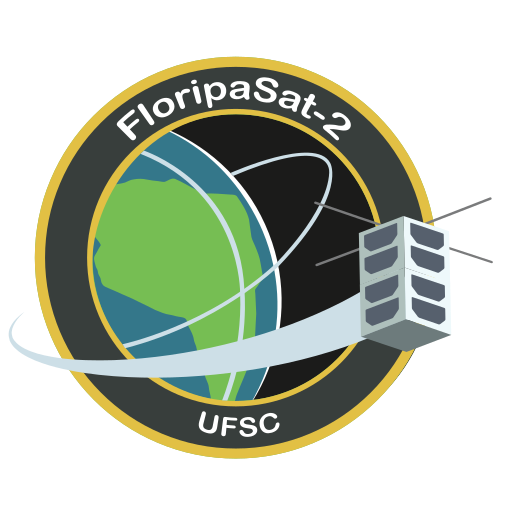
\includegraphics[width=0.5\textwidth]{figures/floripasat2-patch.png}
        \caption{FloripaSat-2 mission patch.}
        \label{fig:mission-patch}
    \end{center}
\end{figure}
